\documentclass[12pt]{article}
\usepackage[english]{babel}
\PassOptionsToPackage{hyphens}{url}
\usepackage{hyperref}
\usepackage[utf8x]{inputenc}
\usepackage{amsmath}
\usepackage{graphicx}
\graphicspath{{images/}}
\usepackage{parskip}
\usepackage{fancyhdr}
\usepackage{vmargin}
\setmarginsrb{3 cm}{2.5 cm}{3 cm}{2.5 cm}{1 cm}{1.5 cm}{1 cm}{1.5 cm}
\usepackage{float}
\usepackage{caption}
\usepackage{subcaption}

\title{Wireless Data Logger for Elevator Traffic}
\author{Arash Ashrafnejad\\
		Redion Xhepa
		}	
\date{\today}			

\makeatletter
\let\thetitle\@title
\let\theauthor\@author
\let\thedate\@date
\makeatother

\pagestyle{fancy}
\fancyhf{}
\rhead{EEE 212 - 1\\ \thedate}
\lhead{Project Proposal\\
	\thetitle}
\cfoot{\thepage}

\begin{document}

%%%%%%%%%%%%%%%%%%%%%%%%%%%%%%%%%%%%%%%%%%%%%%%%%%%%%%%%%%%%%%%%%%%%%%%%%%%%%%%%%%%%%%%%%

\begin{titlepage}
	\centering
    
\includegraphics[scale = 0.3]{Bilkent.png}\\[0.7 cm]
		    	{\LARGE Electrical and Electronics Engineering Department}\\[0.3cm]	
   	{\LARGE EEE 212 - Microprocessors}\\[0.6 cm]
	\rule{\linewidth}{0.2 mm} \\[0.2 cm]
	{ \LARGE \bfseries Term Project Proposal\\ [0.2 cm]
	 \large \thetitle }\\[0.15 cm]
	\rule{\linewidth}{0.2 mm} \\[1.1 cm]
	
	\begin{minipage}{0.4\textwidth}
		\begin{flushleft} \large
			\emph{Member:}\\
			\theauthor
			\end{flushleft}
			\end{minipage}~
			\begin{minipage}{0.4\textwidth}
			\begin{flushright} \large
			\emph{ Student No.} \\
			21500618\\
			21500280\\
			
		\end{flushright}
	\end{minipage}\\[2 cm]
	
	{\large \thedate}\\[2 cm]
 
	\vfill
	
\end{titlepage}


\section{Introduction}
This project is about implementing a long range wireless transmission and logging embedded system for monitoring elevator traffic using height data from high-precision atmospheric sensor together with accurate real time data.\\
The objective is to monitor and log the elevator traffic onto an SD card in order to analyse the data later. The main motivation behind this is to determine an optimized schedule for the elevator program. For example, the schedule for the idle floor (the floor which elevator should wait when there is no request.) can be set to the floor with maximum traffic at that particular time. Therefore determining the floor with maximum traffic (which given enough data can easily be predicted using regression models) can reduce the elevator traffic and save energy and time.
\section{Project Specifications}
The transmitter module is implemented using 8051 microcontroller and the receiver is implemented on Arduino Nano. The main motivation behind having a separate sensing and logging system is to reduce maintenance work. Because the sensing device needs to be installed only once and keeps transmitting continuously. However the logging device needs to be checked at least weekly to study the data. Also this way there could be multiple receiver modules and they can monitor the traffic in real time from anywhere within the building (maximum range is 1000 m). The proposed design schematics are shown in Figure 1 and 2. In addition, the detected floor will be shown with a 8x8 dot matrix display on the sensing module for calibration purposes.

\begin{figure}[H]
\centering
\begin{minipage}{.4\textheight}
  \centering
  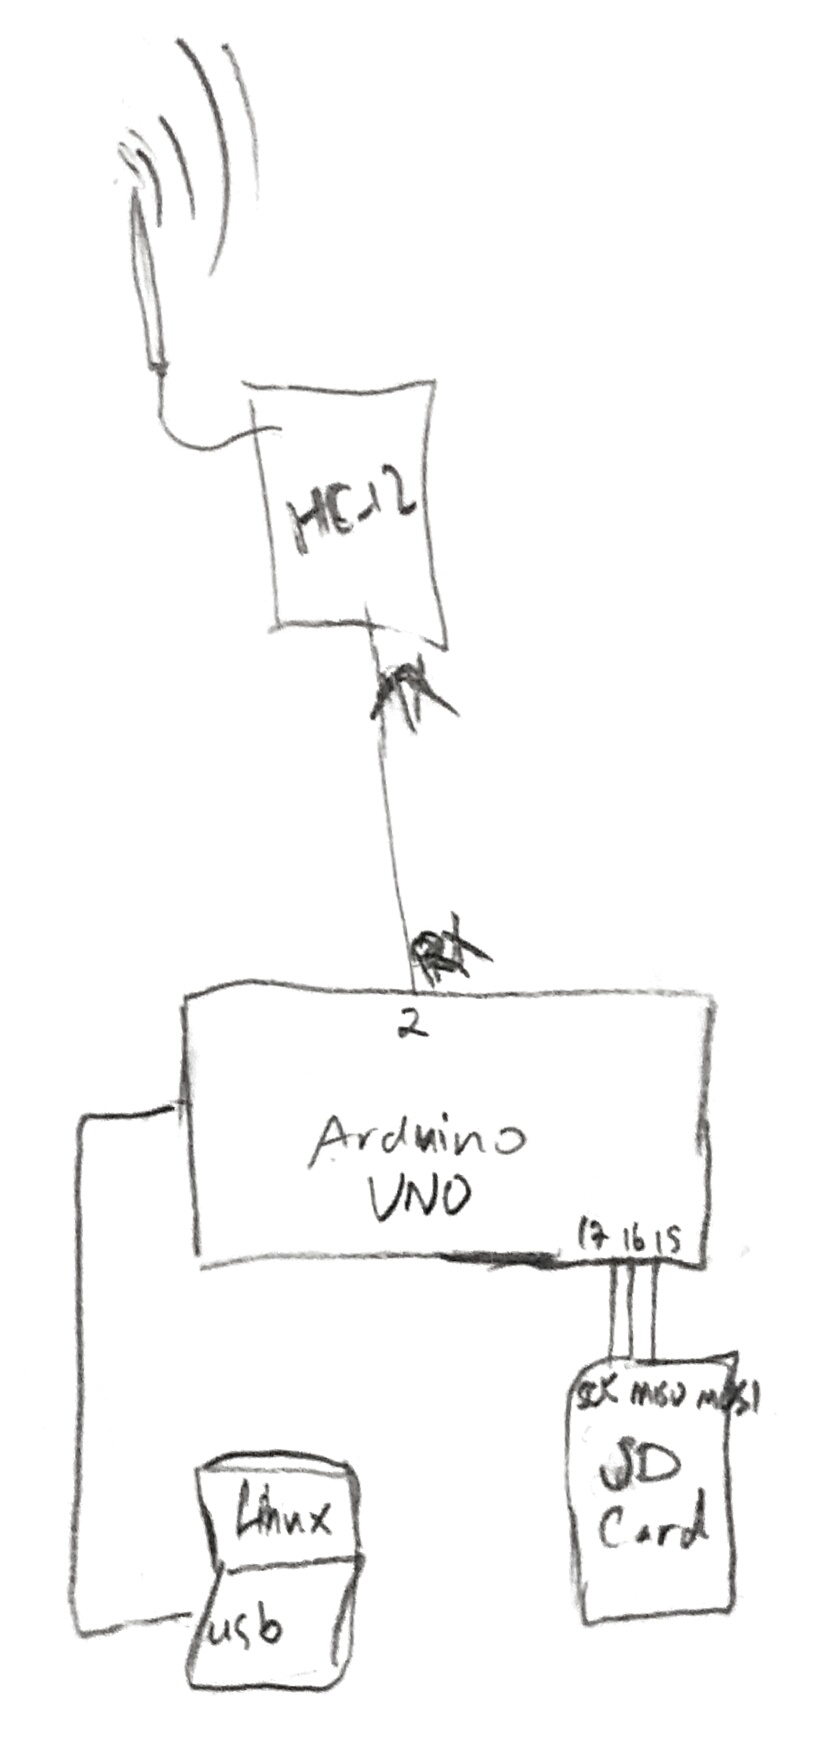
\includegraphics[height=6.3cm]{rx.jpg}
  \captionof{figure}{Receiver Schematic}
  \label{fig:rx}
\end{minipage}%
\begin{minipage}{.4\textheight}
  \centering
  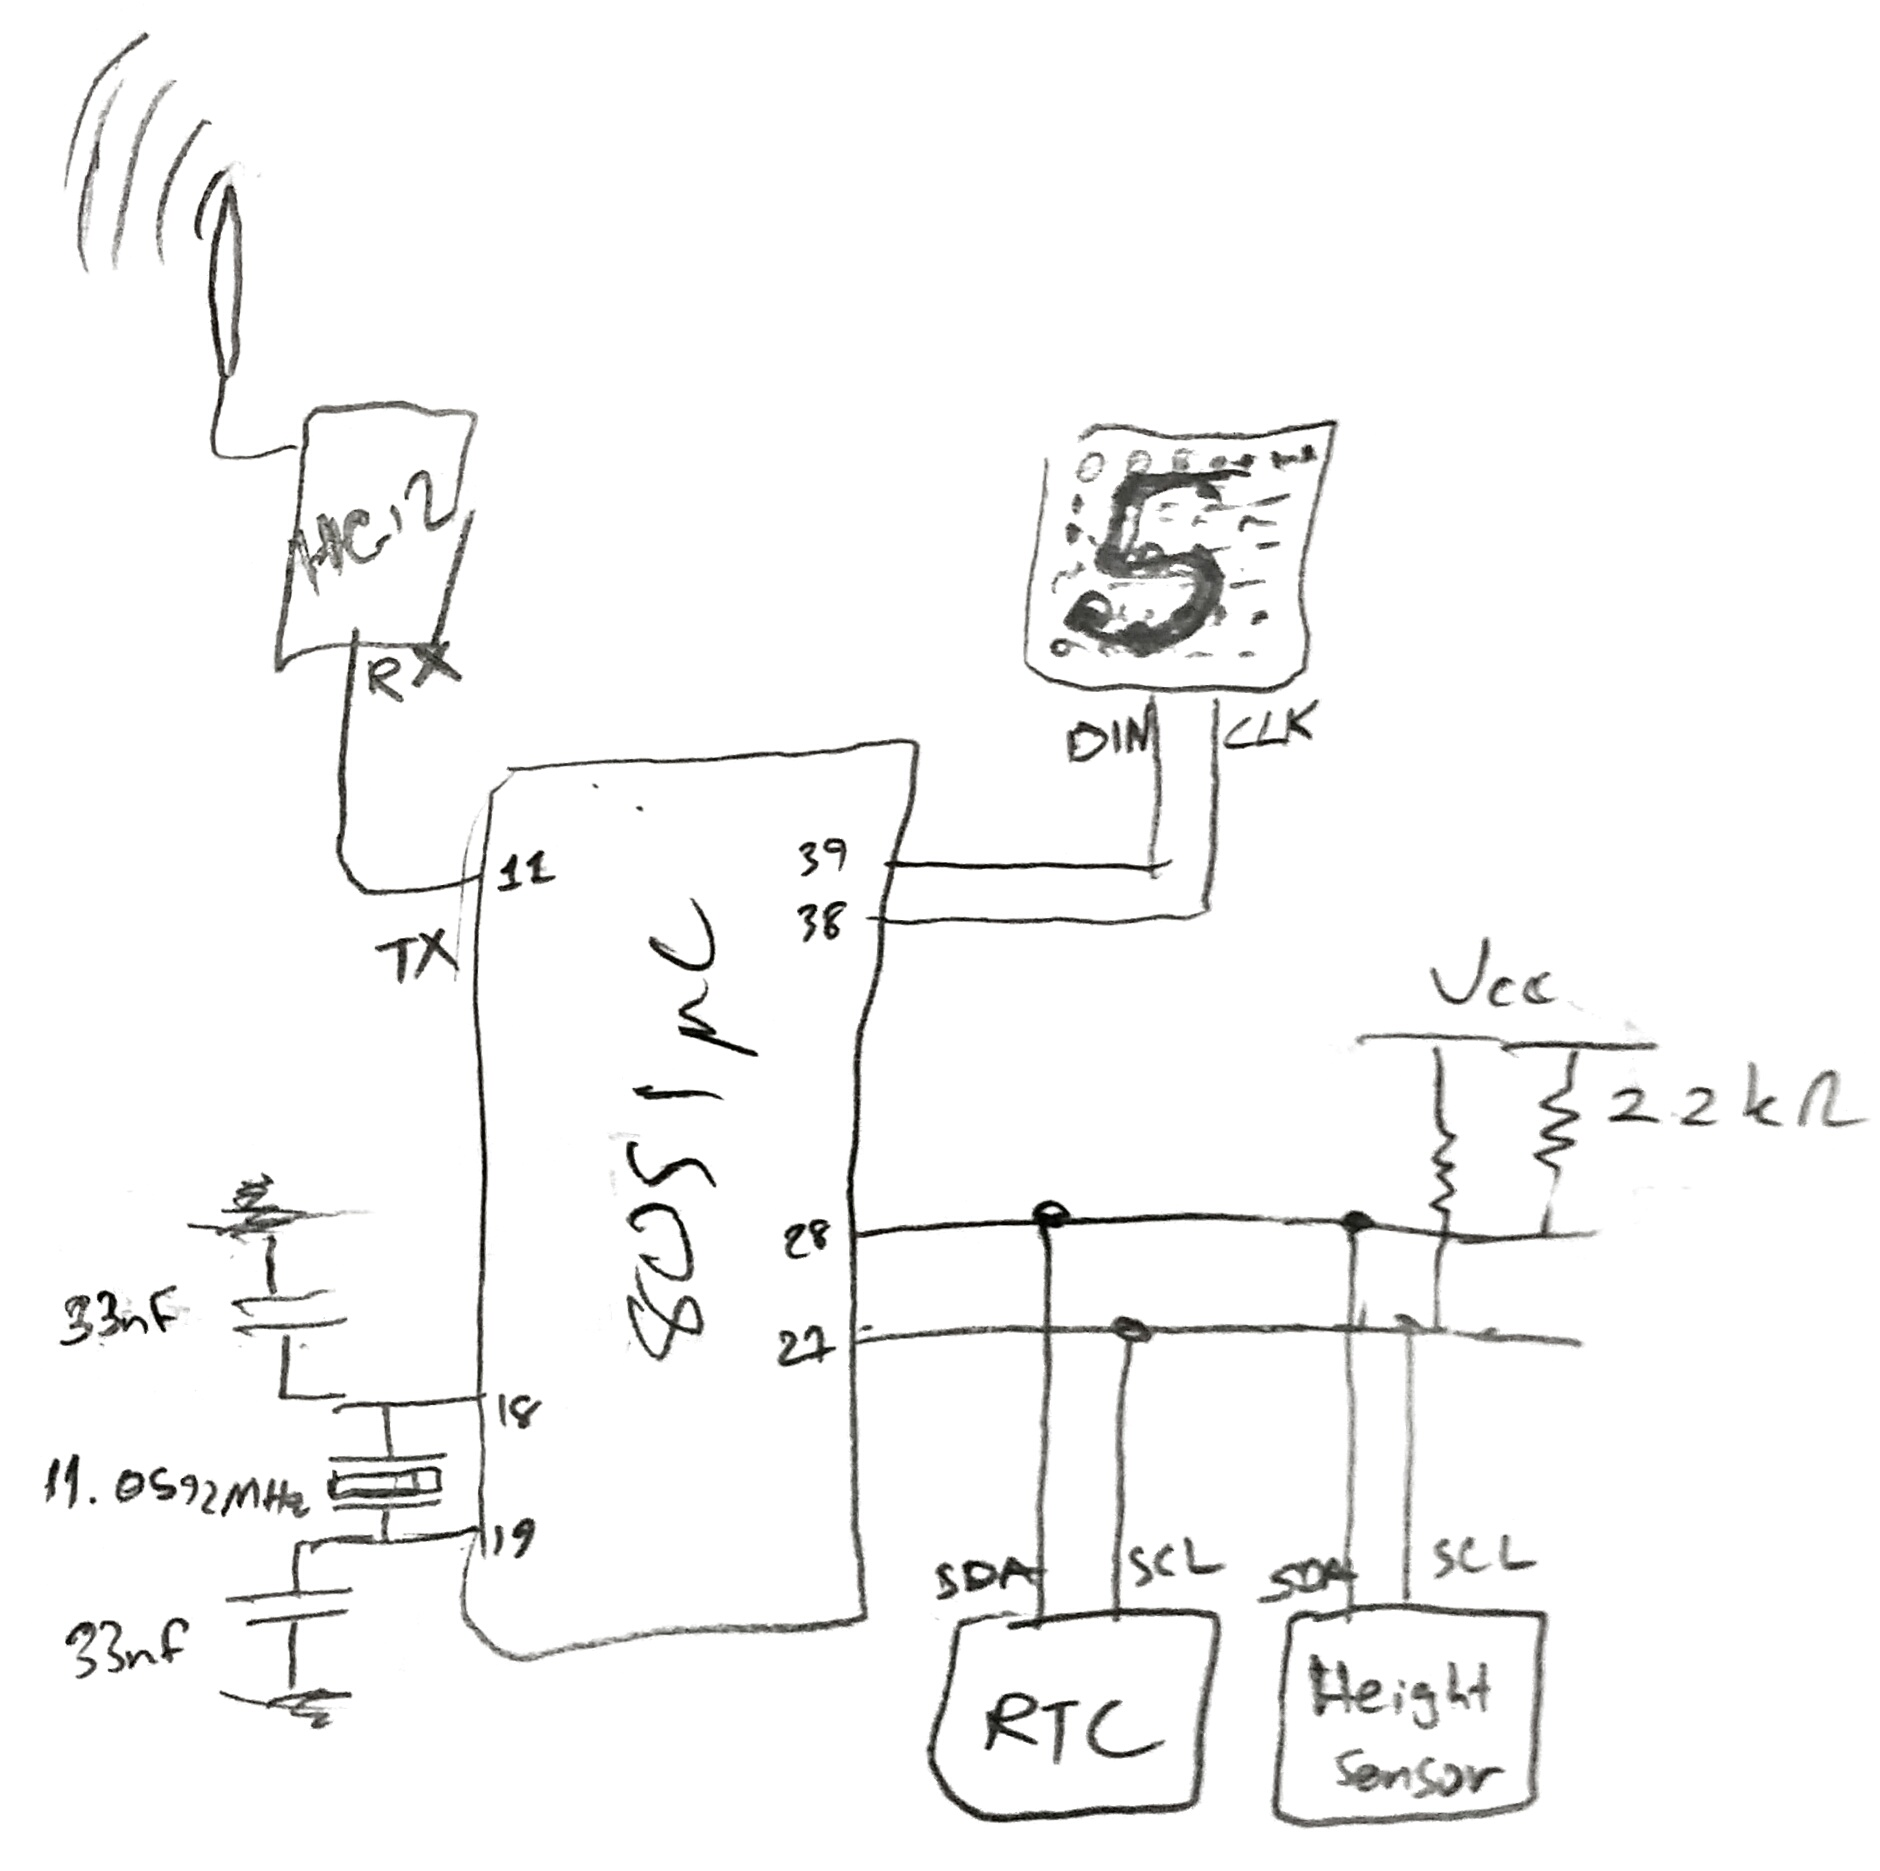
\includegraphics[height=6.3cm]{tx.jpg}
  \captionof{figure}{Transmitter Schematic}
  \label{fig:tx}
\end{minipage}
\end{figure}


\subsection{Required Components}
The list of required components and devices are listed bellow.
\begin{itemize}
\item Breadboard x2
\item Arduino Nano
\item Atmel 8051 Microcontroller
\item HC-12 long-range transceiver x2
\item SMA to IPEX Adapter x2
\item 433 MHz Wireless Radio Antenna x2
\item Micro SD card SPI card reader module  
\item GY-63 Atmospheric Height Sensor Module
\item DS3231 Precision RTC Memory Module
\item MAX7219 Dot Led Matrix Module
\item Breadboard Power Supply Module
\end{itemize}

\begin{figure}[H]
\centering
\begin{minipage}{.4\textheight}
  \centering
  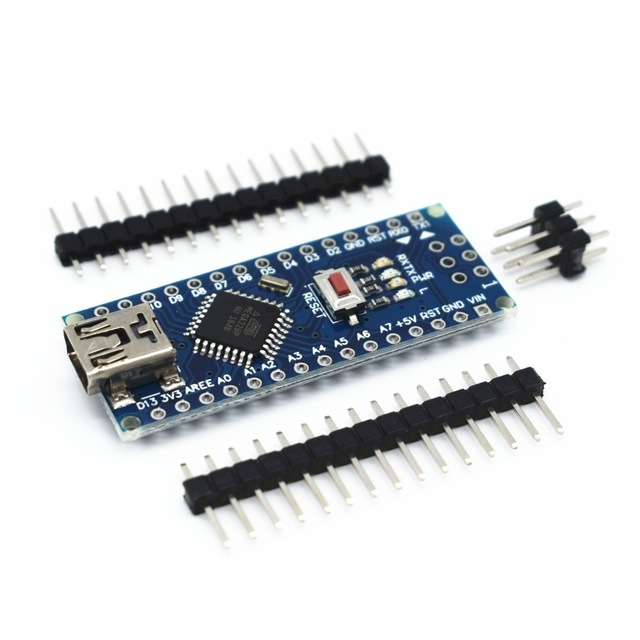
\includegraphics[height=3.5cm]{1.jpg}
  \captionof{figure}{Arduino Nano \cite{1}}
  \label{fig:1}
\end{minipage}%
\begin{minipage}{.4\textheight}
  \centering
  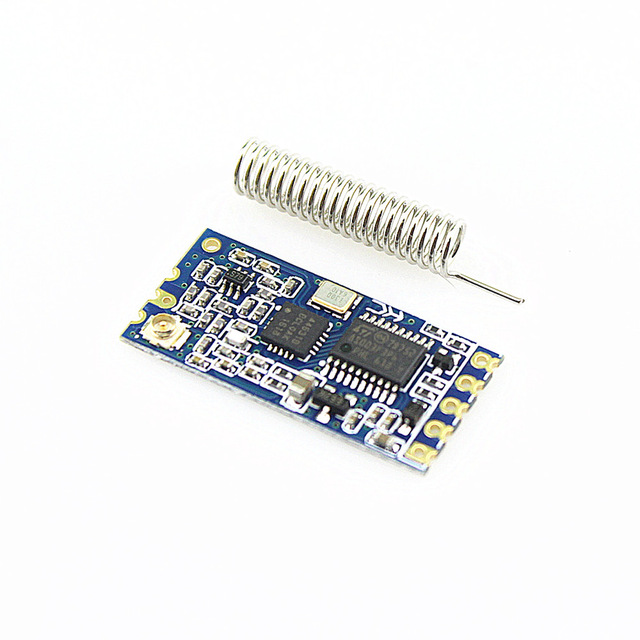
\includegraphics[height=3.5cm]{2.jpg}
  \captionof{figure}{HC-12 long-range transceiver \cite{2}}
  \label{fig:2}
\end{minipage}
\end{figure}

\begin{figure}[H]
\centering
\begin{minipage}{.4\textheight}
  \centering
  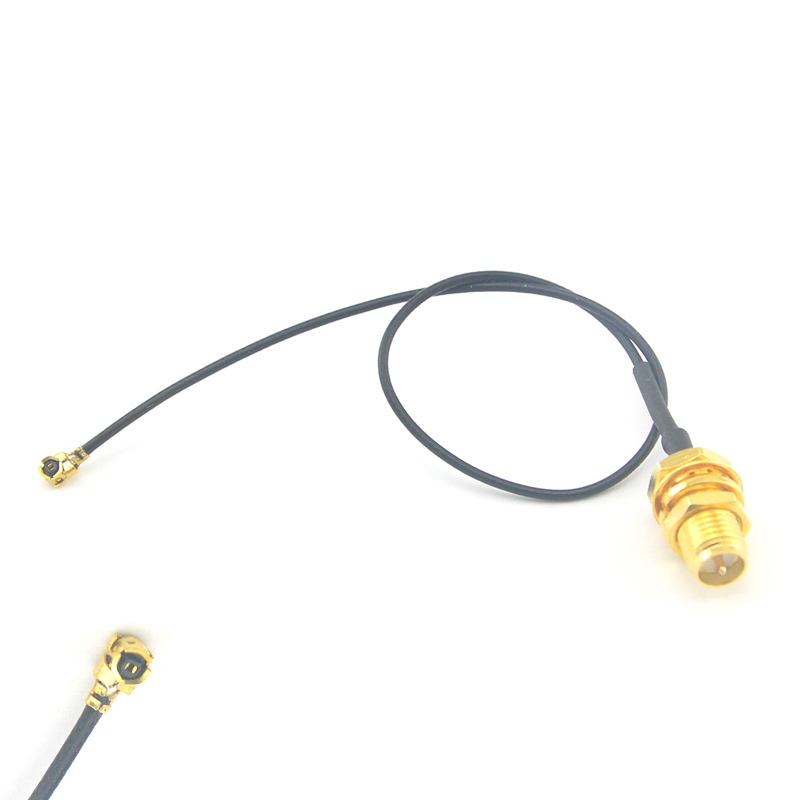
\includegraphics[height=3.5cm]{3.jpg}
  \captionof{figure}{SMA to IPEX Adapter \cite{3}}
  \label{fig:3}
\end{minipage}%
\begin{minipage}{.4\textheight}
  \centering
  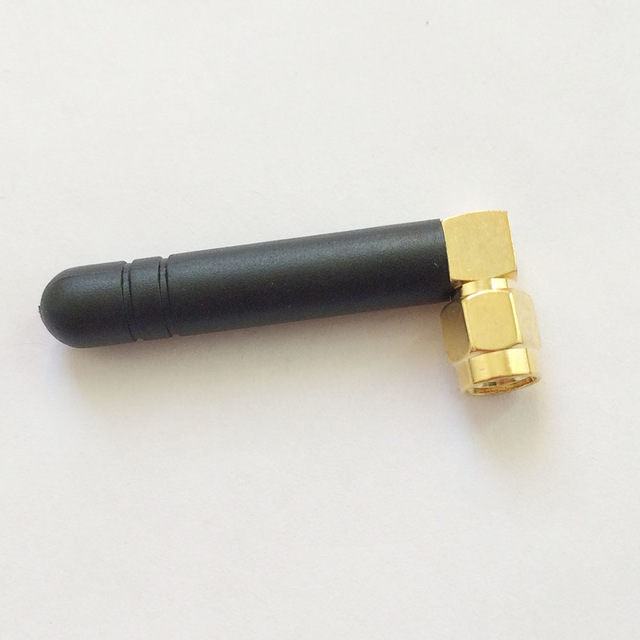
\includegraphics[height=3.5cm]{4.jpg}
  \captionof{figure}{Wireless Radio Antenna \cite{4}}
  \label{fig:4}
\end{minipage}
\end{figure}


\begin{figure}[H]
\centering
\begin{minipage}{.4\textheight}
  \centering
  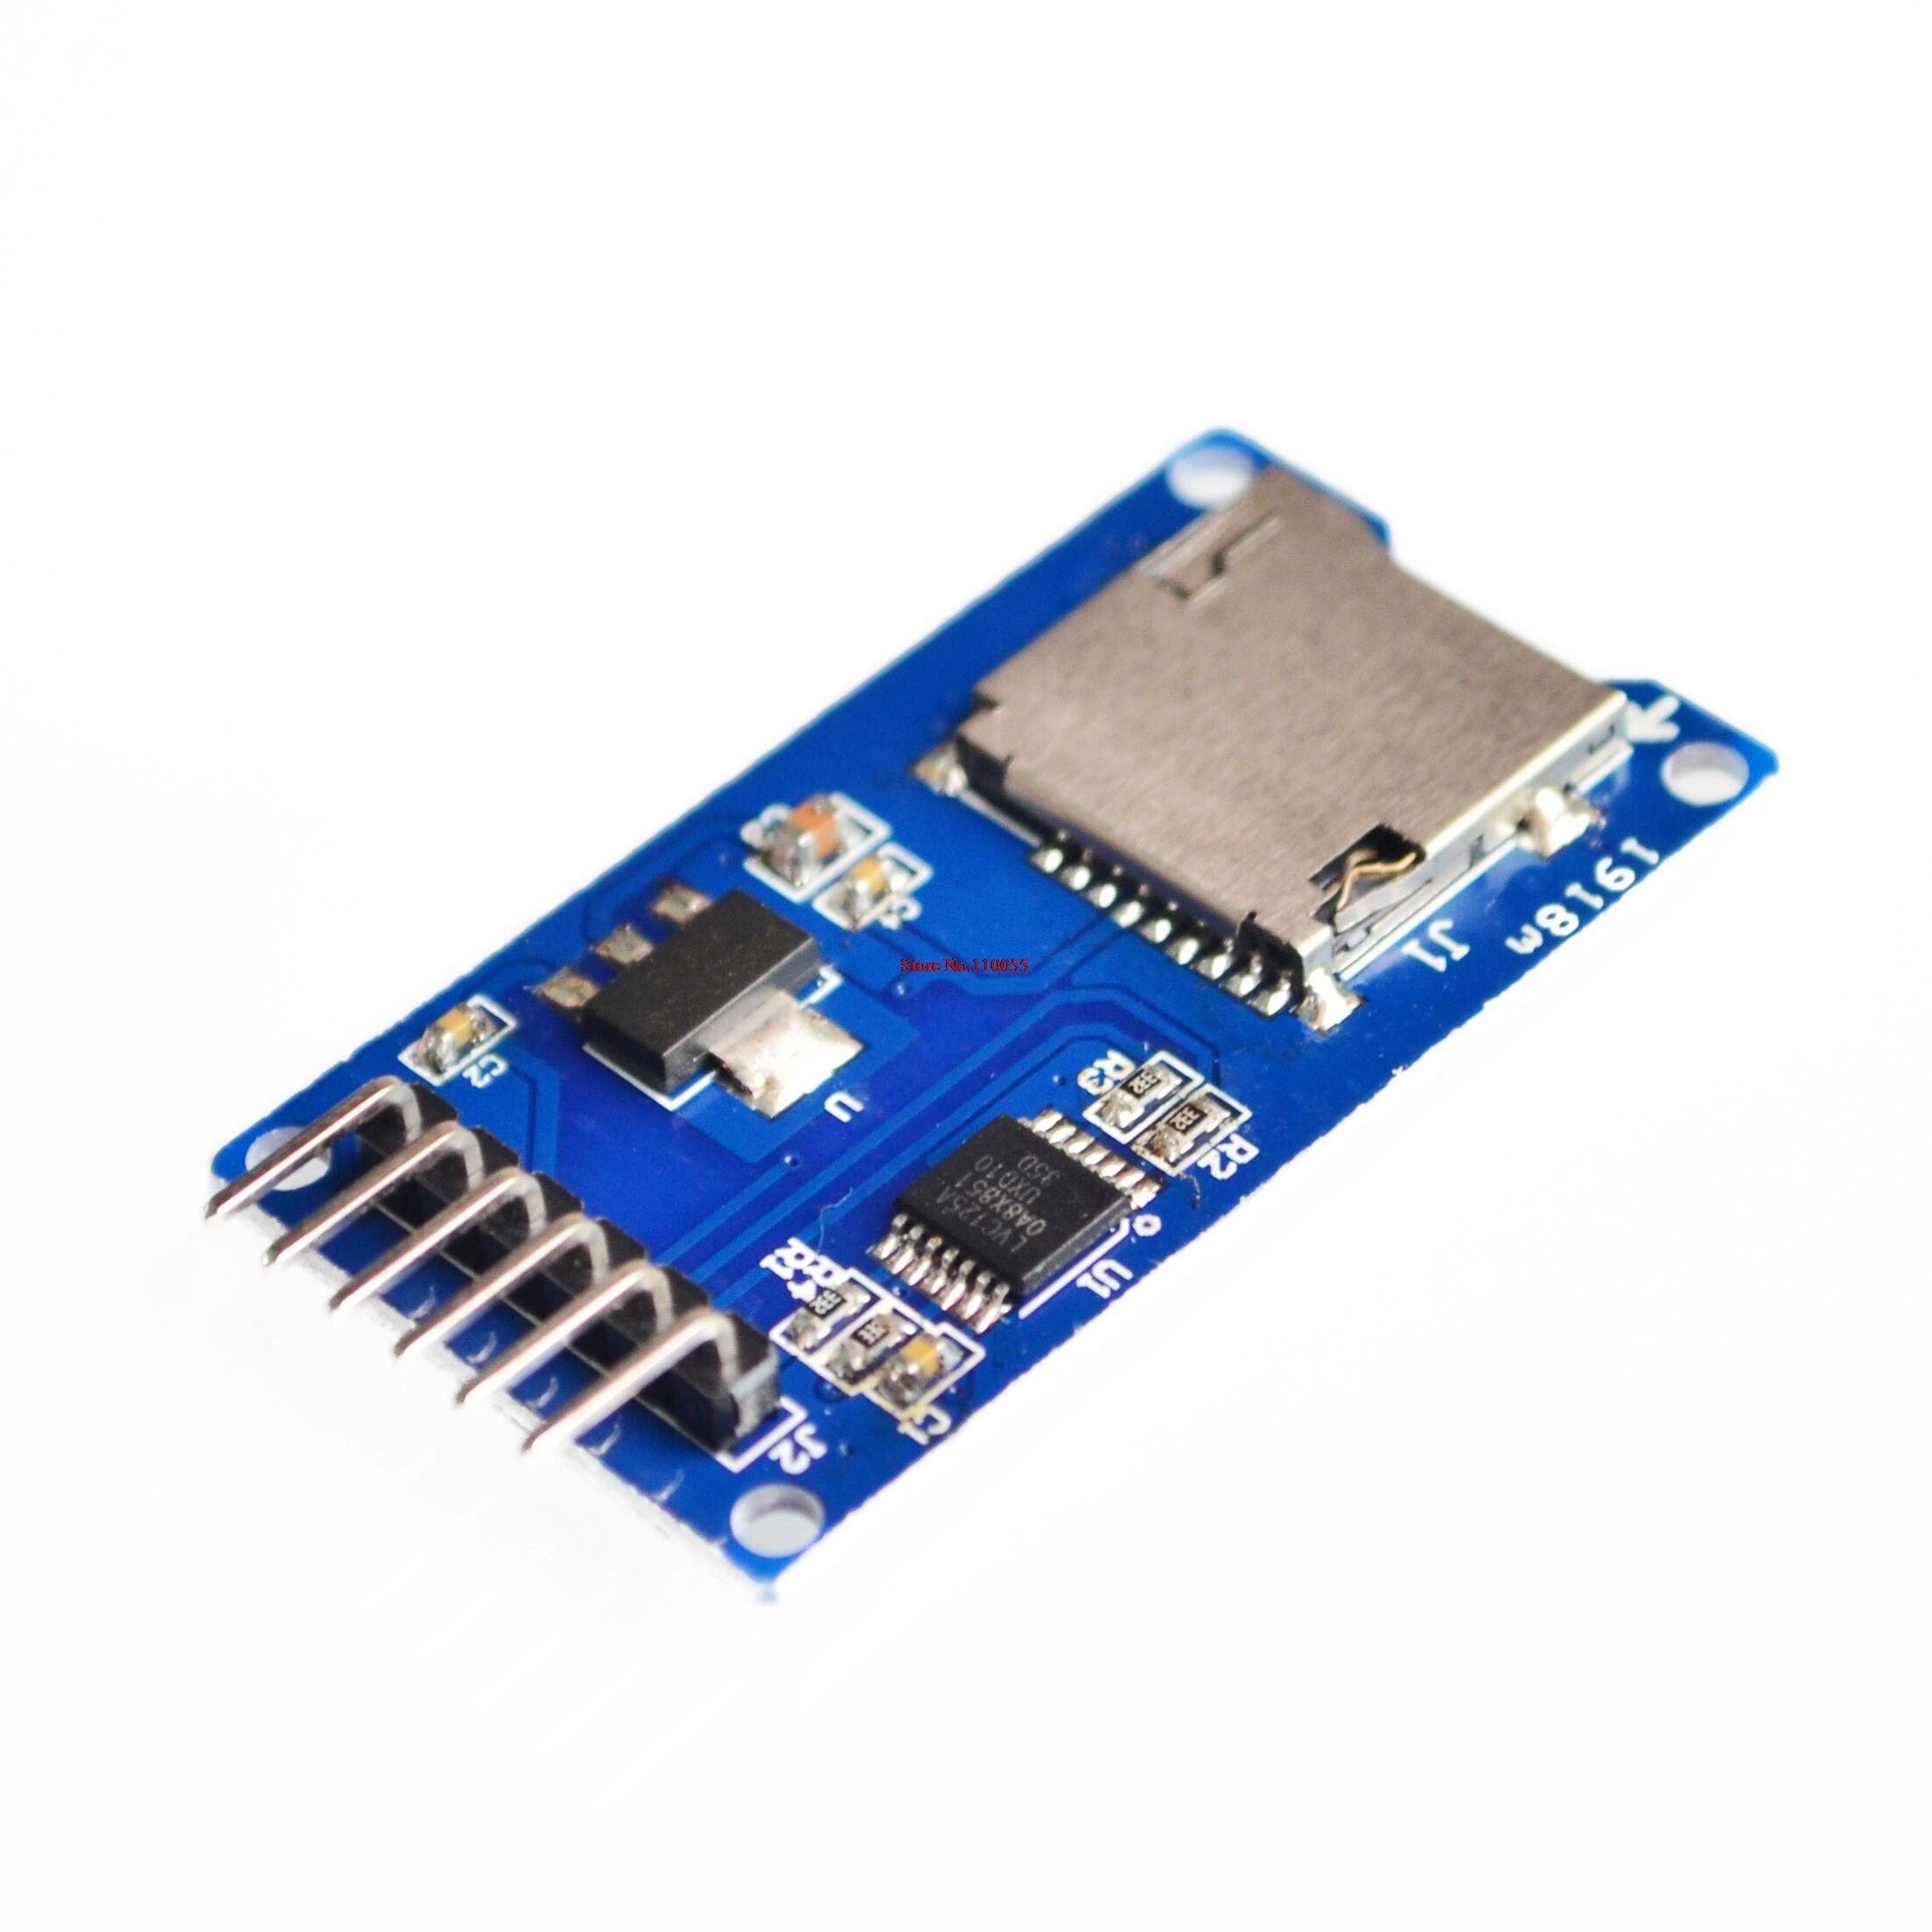
\includegraphics[height=3.5cm]{5.jpg}
  \captionof{figure}{Micro SD card SPI card reader \cite{5}}
  \label{fig:5}
\end{minipage}%
\begin{minipage}{.4\textheight}
  \centering
  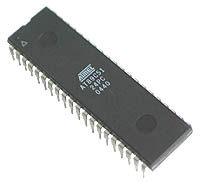
\includegraphics[height=3.5cm]{6.jpg}
  \captionof{figure}{Atmel 8051 Microcontroller}
  \label{fig:6}
\end{minipage}
\end{figure}

\begin{figure}[H]
\centering
\begin{minipage}{.4\textheight}
  \centering
  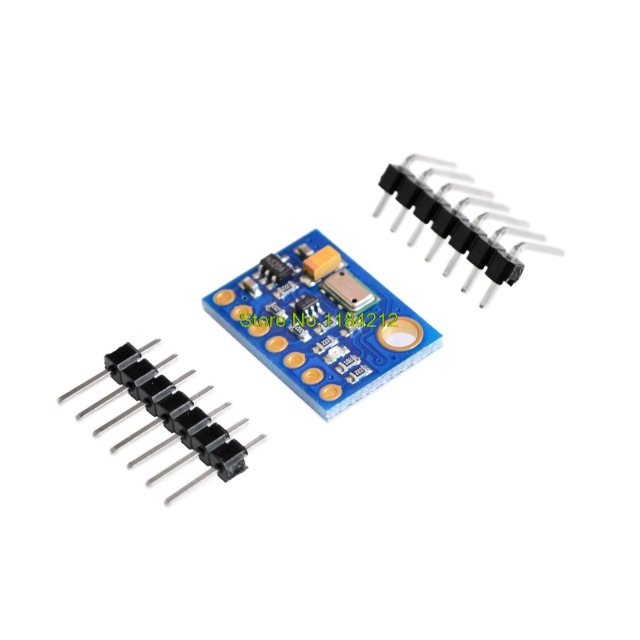
\includegraphics[height=3.5cm]{7.jpg}
  \captionof{figure}{GY-63 Atmospheric Sensor \cite{7}}
  \label{fig:7}
\end{minipage}%
\begin{minipage}{.4\textheight}
  \centering
  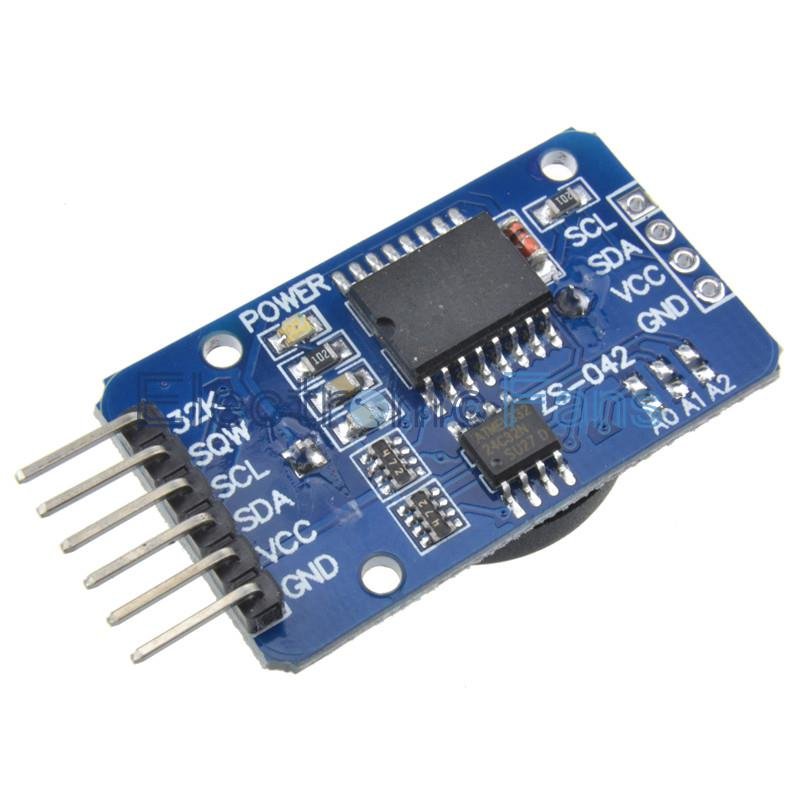
\includegraphics[height=3.5cm]{8.jpg}
  \captionof{figure}{DS3231 Precision RTC Memory \cite{8}}
  \label{fig:8}
\end{minipage}
\end{figure}


\begin{figure}[H]
\centering
\begin{minipage}{.4\textheight}
  \centering
  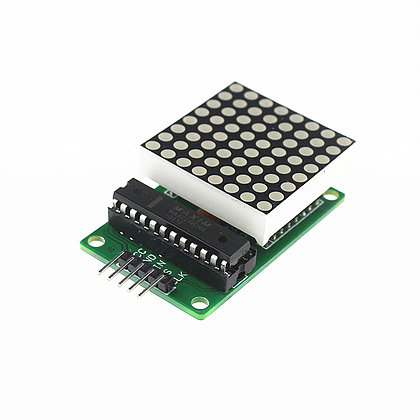
\includegraphics[height=3.5cm]{9.jpg}
  \captionof{figure}{MAX7219 Dot Led Matrix \cite{9}}
  \label{fig:9}
\end{minipage}%
\begin{minipage}{.4\textheight}
  \centering
  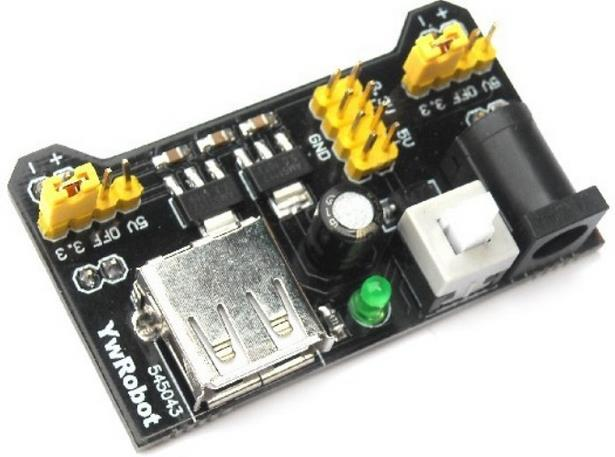
\includegraphics[height=3.5cm]{10.jpg}
  \captionof{figure}{Breadboard Power Supply \cite{10}}
  \label{fig:10}
\end{minipage}
\end{figure}


\newpage
\bibliographystyle{ieeetr}
\bibliography{biblist}
\nocite{*}

\end{document}